% ============================================================
% 03-proposed-model.tex — V13 Architecture (condensed)
% ============================================================
\section{Proposed Model}
\label{sec:model}

This section presents \system{}'s architecture, algorithms, and evidence-acquisition mechanisms. The design follows three principles: \emph{centralized agent coordination} (a contract-checked supervisor dispatches each query to one domain agent); \emph{heterogeneous knowledge allocation} (each information structure maps to a corresponding evidence representation); and \emph{representation-aware evidence routing} (graph-tool or intent-scoped retrieval path according to the assigned domain).

%------------------------------------------------
\subsection{Overall Architecture}
\label{sec:architecture}

Figure~\ref{fig:architecture} illustrates three coordinated tiers: (1)~the Interaction and Centralized Supervisor Tier, (2)~the Domain-Specialized Multi-Agent Core, and (3)~the Heterogeneous Knowledge Storage and Tool Tier.

\begin{figure}[t]
\centering
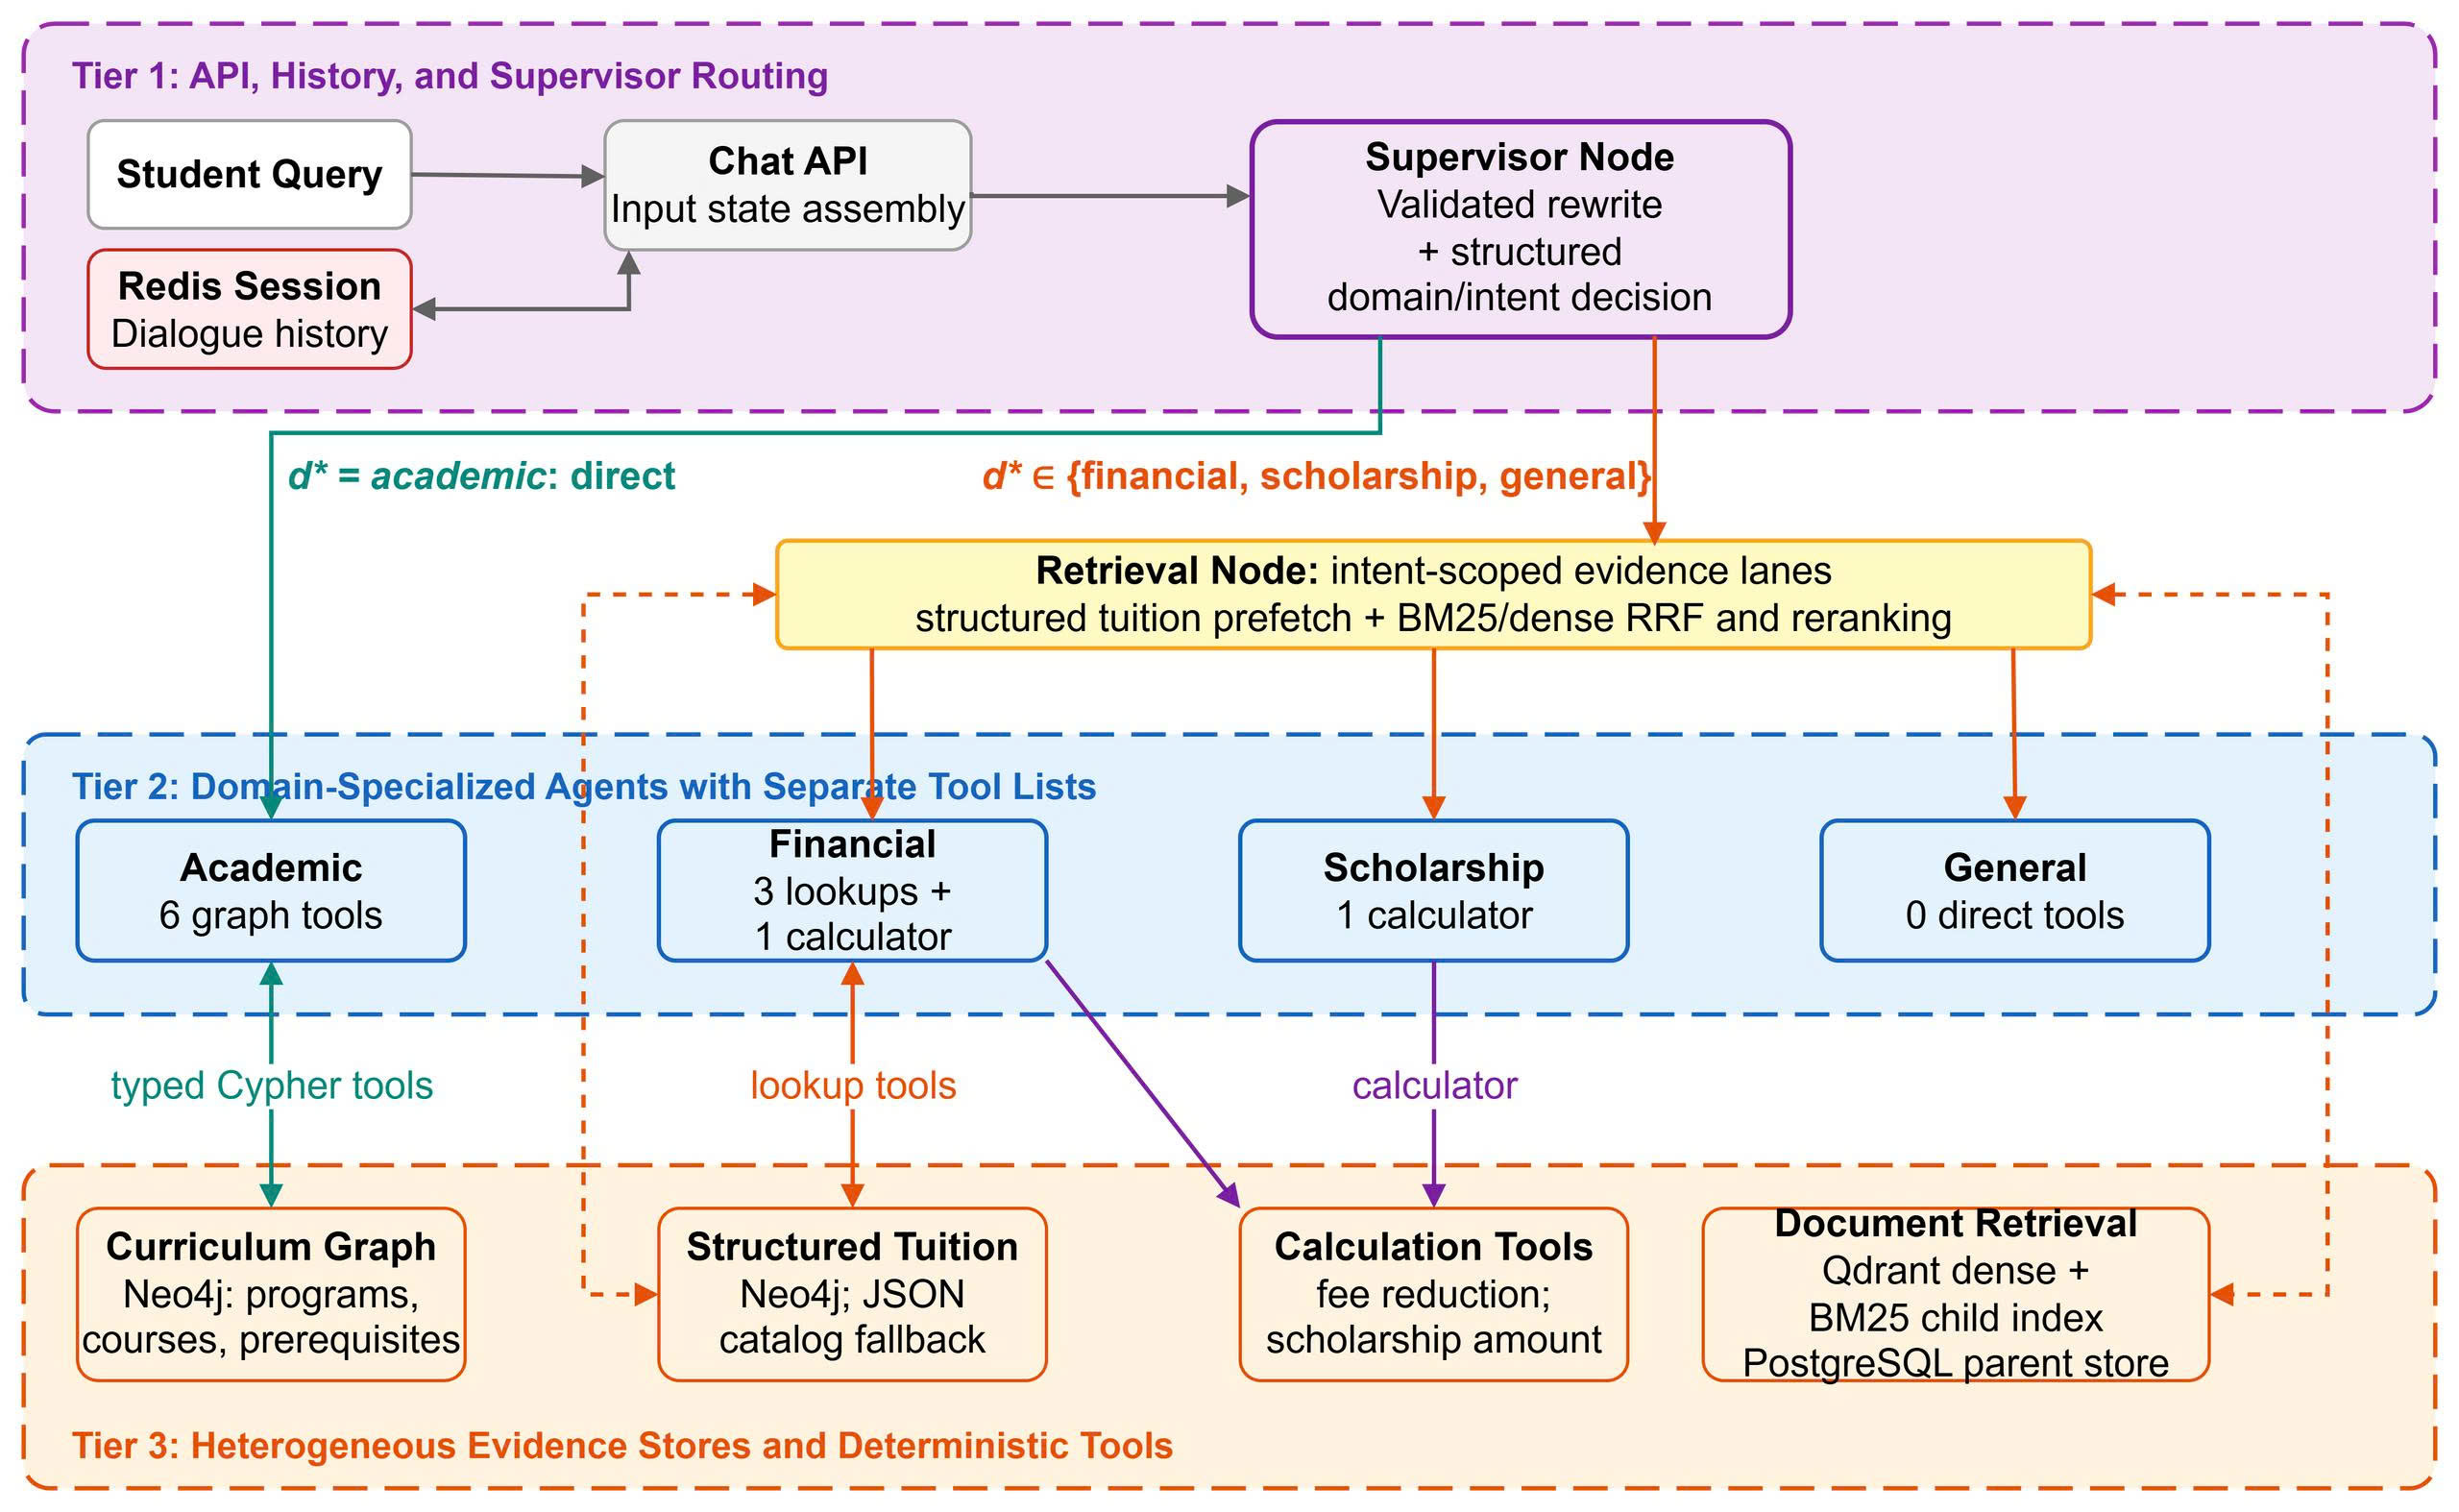
\includegraphics[width=\textwidth]{figures/architecture.jpg}
\Description{Diagram of the three-tier CTU-Chat system architecture. The top tier shows the interaction layer with a centralized supervisor router. The middle tier contains four domain-specialized agents: an academic graph agent connected to Neo4j, a financial agent with deterministic arithmetic tools, a scholarship agent with hybrid retrieval, and a general administrative agent. The bottom tier shows the heterogeneous knowledge storage layer comprising Neo4j graph database, PostgreSQL parent-chunk store, Qdrant vector index, and Redis session history. Solid arrows denote direct tool access and dashed arrows denote retrieval-node evidence acquisition. A contract-repair mechanism validates and may correct the supervisor's routing decision before conditional dispatch.}
\caption{Implemented \system{} architecture. Redis history enters the graph state; the supervisor's structured decision is contract-checked before conditional dispatch. Academic queries enter the graph-enabled agent; other domains pass through intent-scoped retrieval.}
\label{fig:architecture}
\end{figure}

\system{} specializes LangGraph through typed state (\texttt{AgentState} with validated rewrite, routes, evidence, and response), an intent--owner contract that checks structured supervisor output before dispatch, conditional routing (academic queries go directly to the graph agent; others through retrieval), acyclic orchestration (specialists return to \texttt{END} without peer edges), and asymmetric tool registries (each specialist sees only its scoped tools).

%------------------------------------------------
\subsection{Neo4j Knowledge Graph and Cypher Tools}
\label{sec:neo4j_graph}

The Neo4j graph contains over 1,500 nodes and 3,800 edges across 113 undergraduate curricula and fee schedules. Its 10 node labels cover curriculum entities (\texttt{Program}, \texttt{Course}, \texttt{Block}) and tuition entities (\texttt{TuitionFee}, \texttt{TuitionPolicy}, \texttt{ExemptionBasisRate}); 13 typed relationships encode containment, prerequisites, program outcomes, tracks, occupations, tuition, and exemption bases.

The system does not ask the LLM to generate arbitrary Cypher. After the supervisor selects the academic agent, its ReAct policy chooses one of six typed tools and supplies arguments. Each tool normalizes identifiers and calls a fixed, parameterized Cypher query implementing three query classes: \emph{attribute lookup/search} (program codes, names, comparisons), \emph{structural traversal} (prerequisite chains up to ten hops, course intersection, reverse path search), and \emph{structured financial lookup} (tuition, policies, exemption rates). This design binds agent actions to deterministic graph operations, reducing exposure to errors from unconstrained Cypher generation.

%------------------------------------------------
\subsection{Routing and Deterministic Arithmetic}
\label{sec:algorithms}

For a query $q$ and its dialogue predecessor, the supervisor first attempts a validated standalone rewrite, then predicts domain $d_{\mathrm{raw}}$ and intent $\iota_{\mathrm{raw}}$ under a structured schema, falling back to \texttt{general}/\texttt{other} on parsing failure. The ownership contract repairs rule conflicts or incompatible domain--intent pairs. Academic queries proceed directly to the graph agent; other domains build intent-scoped retrieval lanes, with financial queries first attempting Neo4j tuition lookup and then JSON fallback.

\textbf{Deterministic Tuition Arithmetic.}
For fee-reduction requests, the external tool \texttt{tinh\_toan\_hoc\_phi} receives three parameters---per-credit tuition $T$, per-credit exemption basis $B$, and percentage $p$---and applies:
\begin{equation}
  D = B\frac{p}{100}, \qquad P = \max(0, T-D).
  \label{eq:tuition_reduction}
\end{equation}
The tool enforces $0 \le p \le 100$ and clamps $P$ at zero. The contribution lies in composing validated rewriting, constrained routing, and deterministic arithmetic within the multi-agent workflow.

%------------------------------------------------
\subsection{Heterogeneous Knowledge Allocation and Hybrid Retrieval}
\label{sec:hybrid_retrieval}

Rather than a uniform document index, \system{} preserves relational curricula in Neo4j, accesses cohort-dependent tuition through structured lookup, and retains narrative regulations in document retrieval. Academic queries enter the graph agent directly; others enter retrieval. Financial retrieval first attempts Neo4j tuition lookup with JSON fallback; the repaired intent then selects metadata-filtered document lanes.

For narrative regulations and scholarship criteria, BM25 and Qdrant search 400-character child chunks; parent sections (2,800-char target, 100-char overlap) are loaded from PostgreSQL and fused via RRF: $s_{\mathrm{RRF}}(d)=\sum_{s\in\{\mathrm{bm25},\mathrm{dense}\}}(60+r_s(d))^{-1}$. The full stack pools intent-governed and unfiltered candidates, deduplicates, and reranks with \texttt{bge-reranker-v2-m3}. Scores below 0.20 are removed unless fewer than two candidates remain; graph evidence is added under fixed quotas and up to seven passages are packed for generation.

%------------------------------------------------
\subsection{Cross-Domain Query Handling}
\label{sec:cross_domain}

A bounded specialist architecture raises the question of how queries spanning multiple domains are handled. \system{} adopts a \emph{single-owner with multi-evidence prefetch} policy: the supervisor selects one primary owner based on dominant intent, but the retrieval layer collects evidence from all relevant sources before passing aggregated context to the owner. Specialists do not invoke other specialists; if the query requires a tool outside the owner's scope, evidence is prefetched through retrieval rather than cross-specialist delegation. This design trades full cross-domain tool composability for bounded execution. The 20 cross-domain held-out queries directly test this mechanism.
